\chapter{Making numbers trustworthy}\label{ch:trust}

At a site serving only a few families, one family's departure can change the completion rate enough to alter the site's rank. A funder who uses that ranking needs to know how uncertain the rate is. Similar questions arise when we combine survey items into a score, generalize from respondents to a population, or plan a study around an effect that may be hard to detect.

In this chapter we examine survey scales and weights, stabilize small-site rates, and calculate what a planned study can detect. We then build prediction intervals and estimate how much outcome variation remains between sites after accounting for measured predictors. The examples in \texttt{ch07\_trust.do} let you connect each diagnostic to a reporting decision: which comparisons the evidence supports, what uncertainty to show, and what to investigate before publishing.

The safeguards also belong on the calendar before the analysis does, because each failure has its own lead time: a failed reliability check means items rewritten and re-fielded, a survey wave's cost; an unweightable sample means population margins requested from whoever holds them; a power shortfall means a redesign while the budget can still move.\marginnote{Make the checks a working habit: draft a one-page pre-analysis measurement checklist alongside the evaluation plan, give each of the four checks a date and an owner, and schedule reliability and power earliest because their fixes take longest.} If you find an alpha of 0.55 in the final month, all you can do is caveat it; find the same alpha in the pilot and you can still repair it.

A skeptical program officer will ask each of this chapter's questions out loud: does this scale hold together, do these respondents stand in for our clients, is this small site's rate real or an accident of its size, and could this study have found the effect at all. Program teams already trust performance-measurement systems, logic-model indicators, and What Works Clearinghouse evidence tiers, and every one of those systems assumes someone has answered these four questions, so an evaluator who can show that work is speaking their language. The AEA Guiding Principles oblige an evaluator to systematic inquiry and competence on behalf of the people the program serves, and the checks in this chapter are one concrete way to meet those obligations. Table~\ref{tab:ch07-viz-map} lists each safeguard, the skeptical question it answers, and the Stata command that does the work.

\begin{table*}[htbp]
\centering
\caption[The chapter's safeguards and the question each answers]{Read down the middle column for the skeptical program officer's question, then across to the safeguard that answers it and the tool that does the work. The last two rows are newer to evaluation practice, prediction intervals and variance partitioning, and both ship as commands here; model-based small-area estimation, the proposed tool this chapter also names, is not yet one of them.}
\label{tab:ch07-viz-map}
{\footnotesize
\begin{tabular}{p{2.3cm}p{4.7cm}p{2.4cm}}
\hline
Safeguard & The question it answers & Stata tool \\
\hline
Reliable scales & Do these items measure one thing? & \texttt{alpha}, \texttt{factor} \\
Survey weights & Do respondents stand in for the population? & \texttt{svyset}, \texttt{svy:} \\
Rate shrinkage & Is a small site's rate real or an accident of its size? & \texttt{rateshrink} \\
Study power & Could the study find the effect at all? & \texttt{power} \\
Conformal bands & Where will the \emph{next} case land? & \texttt{conformalpred} \\
Variance split & How much of the spread is the site vs.\ the person? & \texttt{mixed}, \texttt{hlmr2} \\
\hline
\end{tabular}
}
\end{table*}

\section{From items to reliable scales}
Before you average six survey items into one score, confirm they measure the same thing, because a scale that does not hold together will not replicate across waves and every comparison built on it inherits that instability. We check reliability before we model. By the end of this section you will be able to read a reliability table one item at a time, decide which item to cut, and say which decisions you can base on the pruned scale and which you cannot. Cronbach's alpha\index{Cronbach's alpha} (\texttt{alpha}\index{alpha@\texttt{alpha}}) summarizes internal consistency;\sidenote{Alpha depends on both the number of items and their covariance. Interpret it alongside the content of the questions and the intended use of the score; a high value can reflect repetitive items and cannot by itself establish validity.} an exploratory factor check\index{factor analysis} (\texttt{factor}\index{factor@\texttt{factor}}) tests whether the items really track one dimension or several; and where item quality varies enough to matter, item response theory\index{item response theory} (\texttt{irt}\index{irt@\texttt{irt}}) models how hard each item is and how much it reveals about the person answering.\marginnote{Also look at the ends of the scale before averaging. If a third of caregivers sit at the maximum on every item, the instrument has a ceiling: it stops measuring exactly where the program hopes to move people, and real gains for the strongest participants vanish into the top box. One \texttt{tabulate} per item shows it in seconds, and the fix is a better instrument, not a different analysis.} The aim is not psychometric perfection but a defensible answer to \enquote{does this scale measure one thing?}

The question a program manager brings is blunt: can I add these six survey items into one \enquote{engagement} score, or is one of them dead weight? To answer it we build a simulated six-item scale for 400 caregivers, five items driven by a shared latent trait and a sixth that barely tracks it, then read \texttt{alpha}:
\par
{\footnotesize
\begin{verbatim}
* simulated: 400 caregivers, one weak item (item6)
set seed 20260704
set obs 400
gen latent = rnormal()
forvalues j = 1/5 {
    gen item`j' = round(3 + latent + rnormal(0, 1))
    replace item`j' = 1 if item`j' < 1
    replace item`j' = 5 if item`j' > 5
}
gen item6 = round(3 + 0.15*latent + rnormal(0, 1))
alpha item1-item6, item
\end{verbatim}
}
With the \texttt{item} option you get a diagnosis rather than a single coefficient, one row per item:
\par
{\footnotesize
\begin{verbatim}
Test scale = mean(unstandardized items)
                    Item-test  Item-rest  interitem
Item     Obs  Sign  corr       corr       cov       alpha
item1    400   +     0.7155     0.5475    .4687989  0.7086
item2    400   +     0.7470     0.5961    .4522575  0.6950
item3    400   +     0.6954     0.5266    .4847419  0.7147
item4    400   +     0.7299     0.5777    .4664480  0.7009
item5    400   +     0.7290     0.5656    .4598596  0.7034
item6    400   +     0.3821     0.1760    .6639919  0.7939
Test scale                                .4993496  0.7576
\end{verbatim}
}
The whole-scale alpha is 0.7576, just over the 0.70 floor, so a manager glancing at the bottom line would ship all six items. Read the item rows, though, and you would not. Item~6 correlates only 0.18 with the rest of the scale where the others sit near 0.55, and the last column reports the result: drop item~6 and alpha rises to 0.7939. Dropping any of the other five would lower it. Refitting on the five good items confirms the number:
\par
{\footnotesize
\begin{verbatim}
. alpha item1-item5
Number of items in the scale:            5
Scale reliability coefficient:      0.7939
\end{verbatim}
}
As a check on the simulation itself, we gave item~6 a latent-variable coefficient of 0.15, compared with 1 for the other items, so it has a weaker relationship with the latent variable than the other items, and the \enquote{alpha if item dropped} column caught exactly the item we planted for it to catch.\marginnote{Read the item-rest correlation before the alpha column: it is the honest signal, since it correlates each item against the \emph{other} items only, not against a total the item helped build. Anything under about 0.30 is a candidate for the cut.} A shorter score may be more internally consistent here, but comparability across waves still requires checking item wording, coding, and how the items behave in each wave.

Before adopting the shorter scale, read item~6 with the program team. Check whether its wording is reversed, whether its coding matches the other items, and whether it measures a part of engagement that the remaining questions omit. A higher alpha supports greater internal consistency in this sample; it does not establish that the scale measures engagement accurately or works equivalently across cohorts. If you revise the score, document the retained items and the rule for handling unanswered questions, then examine the revised scale in the next pilot before comparing waves. That gives the program officer a reasoned scoring decision rather than a cutoff treated as permission to use the score.

\subsection{Fixing a low alpha before the wave closes}\label{sec:alpha-fix}
What do you do with a low alpha? Usually the answer depends on how much of the calendar is left. When the item-rest column shows a single offender and the remaining items still cover the construct, as here, drop the weak item; that fix is the cheapest. When every item limps, or the scale is already too short to prune, rewrite the items and re-field them, which you can only do while a wave remains, the lead-time argument for running \texttt{alpha} on the pilot. When the data are final, all that is left is to report with a caveat, and you will then need to attach that caveat to every table the scale feeds.

\section{Weights that restore the population}\label{sec:weights}
The people who answer a survey are rarely a miniature of the population you need to describe, and any rate you quote from them inherits the mismatch. When you weight the sample back into the population's shape, you close that gap before the rate goes out the door. By the end of this section you will be able to weight a sample back to known population margins, report a rate that describes the people the program serves rather than the subset who answered, and show a board how far those two numbers sit apart before either one goes into a report. We declare the sampling design with \texttt{svyset}\index{svyset@\texttt{svyset}} so that standard errors respect it, then adjust the weights to match known population margins, the census or administrative totals you trust for age, sex, or region, through post-stratification\index{post-stratification} or raking\index{raking}.\marginnote{Raking (iterative proportional fitting) matches several margins at once, e.g. age, sex, and region, when you lack the full joint distribution the cells of post-stratification would need. Watch the extreme weights it can produce: a handful of respondents carrying weights of 40 or more will quietly wreck your effective sample size.} Here is where the nonresponse diagnostics of Chapter~\ref{ch:surveys} pay off: the imbalance those tests detect is the imbalance these weights repair.

The question is whether weighting changes the headline number enough to matter. Stata ships the NHANES~II survey, which deliberately oversampled older adults, so it is the cleanest place to see the gap.\marginnote{Once you \texttt{svyset} the design, let Stata apply it for you: prefixing an estimation command with \texttt{svy:} propagates the strata and weights into every standard error. Applying \texttt{[pweight=]} to individual commands instead gets the point estimate right, but the standard errors those commands print ignore the strata and the clustering.} We take the raw sample mean of a hypertension flag, then declare the design and take the design-based mean:
\par
{\footnotesize
\begin{verbatim}
webuse nhanes2f, clear
mean highbp
svyset psuid [pweight=finalwgt], strata(stratid)
svy: mean highbp
\end{verbatim}
}
Read the \texttt{svyset} line as the design's three facts: \texttt{psuid} names the primary sampling units, the clusters drawn first; \texttt{strata(stratid)} names the layers the draw happened within; and the \texttt{pweight} records how many population members each respondent stands for.

The two estimates are not close. The unweighted mean is 0.4229 and the design-based mean is 0.3687, a gap of 5.4 percentage points on the same 10{,}337 respondents.\marginnote[-15mm]{The reason the gap opens is visible in a second variable: mean age falls from 47.6 unweighted to 42.2 once the weights are applied, because the survey drew extra older adults and hypertension climbs with age.} Table~\ref{tab:weights} lays the two columns side by side.

\begin{table*}[htbp]
\centering
\caption[Weighted versus unweighted means, NHANES~II]{Unweighted sample means versus design-based (weighted) means, NHANES~II, $N=10{,}337$. The survey oversampled older adults, so the raw sample skews old and hypertensive; the weights restore the population age structure and the hypertension rate falls with it.}
\label{tab:weights}
{\footnotesize
\begin{tabular}{lccc}
\hline
Measure & Unweighted & Weighted & Gap \\
\hline
High blood pressure (share) & 0.4229 & 0.3687 & $-0.054$ \\
Age (years)                 & 47.56  & 42.24  & $-5.33$ \\
\hline
\end{tabular}
}
\end{table*}

The direction of the gap is the check that the weights are working: the oversampled older adults carry more hypertension, so the raw average overstates the population rate, and the weights pull it back down.\marginnote{In policy units the gap is not academic: a state health office reporting \enquote{42\% of adults have high blood pressure} when the weighted figure is 37\% overstates the rate by five percentage points, the kind of gap that misdirects a screening budget applied to a population of millions.} Funders and boards do not quote \enquote{our respondents said}; they quote \enquote{our participants are}. Weighting lets you make that second, population-level claim honestly, so the reported number describes the program's people rather than the subset who happened to answer.

Give the program officer the same pairing of finding and license: \enquote{37\% is the rate for the people we serve; 42\% describes only who answered.} Before quoting either figure, compare the two. When weighting barely moves the estimate, say so; that stability shows limited sensitivity to these particular weights, although bias related to unmeasured differences may remain. When it moves the estimate this much, lead with the weighted number and park the unweighted one in an appendix. Inspect the distribution of relative weights and the effective sample size before publishing. Absolute weight values depend on their normalization; a value of 40 is not by itself a reason to trim. If a few respondents dominate the weighted estimate, investigate their cells and compare results under a documented trimming rule.

\section{Stabilizing noisy small-site rates}\label{sec:shrink}
Rates computed on tiny denominators are wild by construction, and in an evaluation those wild rates drive real funding and blame. A single failure at a five-person clinic can drop it to the bottom of a ranking that decides its budget, even though the estimate contains almost no information. We fix that with empirical Bayes shrinkage\index{empirical Bayes shrinkage}, because\marginnote{The statistician's name for this is \enquote{borrowing strength}: each small site quietly leans on the whole distribution of sites to estimate its own rate. It is the same machinery behind Stein's paradox, the 1950s discovery, given its explicit shrink-toward-the-center form by James and Stein in 1961, that pooling several noisy estimates beats taking each at face value.} it pulls extreme low-$N$ rates toward the regional mean in proportion to how little data supports them, so a site with five cases is nudged hard toward the average while a site with five hundred barely moves. You retain each site's observed rate and report the adjusted estimate alongside it, so readers can see how much pooling changed the result.

We simulate 50 sites with caseloads from 5 to 500, most of them small, and true completion rates centered near 0.20. A beta-binomial moment estimator reads the blend weight straight off the observed mean and spread of the site rates, no iterative fitting, and gives each site a shrunken rate: a caseload-weighted blend of its own raw rate and the grand mean. Written out, that blend is
\begin{equation}
  \hat p_i \;=\; \frac{y_i + M\bar p}{n_i + M}
           \;=\; w_i\,\frac{y_i}{n_i} + (1-w_i)\,\bar p,
  \qquad
  w_i \;=\; \frac{n_i}{n_i + M},
  \label{eq:ch07-viz-shrink}
\end{equation}
where $y_i$ is the site's successes, $n_i$ its caseload, $\bar p$ the grand mean across sites, $M$ the prior sample size the estimator fits, and $w_i$ the weight placed on the site's own data. Everything follows from that weight: a five-person site has $w_i$ near zero and is nearly all prior, while a $500$-person site has $w_i$ near one and barely moves. The Stata block below computes exactly this, with \texttt{M*pbar} standing in for the numerator's $M\bar p$:
\par
{\footnotesize
\begin{verbatim}
* simulated: 50 sites, caseloads 5-500, rates ~ 0.20
set seed 20260704
set obs 50
gen n     = 5 + int(495*runiform()^2)
gen ptrue = rbeta(8, 32)
gen y     = rbinomial(n, ptrue)
gen praw  = y/n
quietly summarize praw
scalar pbar = r(mean)
scalar s2   = r(Var)
gen sampv   = pbar*(1 - pbar)/n
quietly summarize sampv
scalar tau2 = max(s2 - r(mean), 1e-6)
scalar M    = pbar*(1 - pbar)/tau2 - 1
gen pshrunk = (y + M*pbar)/(n + M)
\end{verbatim}
}
The two constants that drive the blend are a grand mean of 0.195 and a prior sample size $M$ of 32.4\marginnote{A prior sample size $M$ of 32.4 means every site is treated as if it came with an extra 32 cases pinned at the grand mean.}. When we sort by how far each site moved, the mechanism shows up at its most extreme:
\par
{\footnotesize
\begin{verbatim}
. list site n praw pshrunk move in 1/3, noobs
  site    n    praw   pshrunk     move
    26    7   0.000     0.160    0.160
    11   15   0.400     0.260   -0.140
     3    6   0.333     0.217   -0.117
\end{verbatim}
}
Site~26 is the mechanism in one row: it recorded zero successes out of seven and would rank dead last on the raw rate, but seven cases cannot support a claim of \enquote{never,} so shrinkage lifts it to 0.160, near the pack. Site~11 posted 0.400 on only 15 cases and is pulled down to 0.260. In every case the move is large precisely because the denominator is small; no site with a caseload in the hundreds appears in this list. Figure~\ref{fig:shrink} plots all 50 at once, and the smallest markers are the ones that moved farthest.

\begin{figure*}[htbp]
\centering
\par
{\footnotesize
\begin{verbatim}
twoway (function y = x, range(0 `pmax')                   ///
            lcolor(gs10) lpattern(dash))                  ///
       (scatter pshrunk praw [aweight=n],                 ///
            msymbol(Oh) mcolor(navy)),                    ///
    yline(`pb', lcolor(cranberry) lpattern(shortdash))
\end{verbatim}
}

\includegraphics[width=\linewidth]{ch07_shrink.png}
\caption[Empirical-Bayes shrinkage of small-site rates]{Raw versus empirical-Bayes rates for 50 simulated sites; marker area is caseload. Points on the dashed 45-degree line did not move; the vertical distance from that line to each marker is the shrinkage. Small markers (tiny caseloads) sit far off the line and are pulled hard toward the grand-mean line at 0.195; the large markers barely budge. The three most-moved sites listed above are all small denominators. Built by \texttt{ch07\_trust.do}.}
\label{fig:shrink}
\end{figure*}

\subsection{Reliability and shrinkage are one number}\label{sec:relid}
The moment estimator above is the teaching version, written out so the blend is visible. The \texttt{rateshrink}\index{rateshrink@\texttt{rateshrink}} package does the same empirical-Bayes fit in one command, adds a posterior interval, and reports a per-unit reliability that is the same shrinkage factor under a different name.

\begin{kaobox}[frametitle=Package Integration: \texttt{rateshrink}]
\texttt{rateshrink} fits empirical-Bayes (Beta-binomial or Poisson-gamma) shrinkage estimates for local rates, turning noisy administrative fractions into stable metrics for dashboards and benchmarking. Install it from the book's public repository:
\par
{\footnotesize
\begin{verbatim}
local gh "https://raw.githubusercontent.com/ericabooth"
net install rateshrink, ///
    from("`gh'/rateshrink-stata-public/main/") replace force
\end{verbatim}
}
Give it the successes, the denominator, and a name for the shrunken column; \texttt{ci()} adds a posterior interval and \texttt{rel()} writes each unit's reliability.
\end{kaobox}

On a fresh 50-site draw, the one-line call reproduces the manual blend and adds the two extras the by-hand code did not:
\par
{\footnotesize
\begin{verbatim}
* simulated: 50 sites
clear
set seed 20260706
set obs 50
gen n = 5 + int(495*runiform()^2)
gen y = rbinomial(n, rbeta(8, 32))
rateshrink, success(y) denominator(n) ///
    generate(pshrunk) ci(95) rel(reliab)
\end{verbatim}
}
The header prints the fitted prior as $\alpha=24.4$, $\beta=89.1$, a prior sample size of 113.5, and the most-moved site as a raw 0.000 pulled to 0.206\marginnote{A raw 0.000 pulled to 0.206 is the same kind of hard lift shrinkage gave Site~26's zero-out-of-seven earlier in the chapter.}. The \texttt{rel()} column adds a useful diagnostic: it reports each site's reliability as $n/(n+\alpha+\beta)$, and on this draw the mean is 0.48, so across these mostly small sites the raw rate contains under half the information a fully reliable measure would.

Read that reliability column again and you are reading this section's shrinkage under another name. \textcite{field2026betabin} prove that a unit's Beta-binomial reliability equals the empirical-Bayes weight placed on its own data, so the fraction $n/(n+M)$ that decides how far a site is pulled toward the mean \emph{is} that site's reliability:
\begin{equation}
  \operatorname{rel}_i
    \;=\; \frac{n_i}{n_i + \alpha + \beta}
    \;=\; \frac{n_i}{n_i + M}
    \;=\; w_i,
  \qquad M = \alpha + \beta,
  \label{eq:ch07-viz-relid}
\end{equation}
with $\alpha,\beta$ the fitted Beta prior's two parameters (so their sum is the prior sample size $M$) and $w_i$ the same shrinkage weight as in Eq.~\eqref{eq:ch07-viz-shrink}. When the fitted weight is 0.5, the adjusted estimate gives equal weight to the site rate and the prior mean. Reliability here names that model-based weight; it is not a probability that the site rate is correct. The authors frame this as a more coherent alternative to the Adams signal-to-noise reliability, the between-site share of total variance long used for healthcare quality measures. The empirical-Bayes tradition running back to \textcite{efron1975data} and Stein's paradox makes the identity intuitive: borrowing strength and discounting for unreliability are one move.\marginnote{\texttt{rateshrink}'s \texttt{rel()} is defined for the Beta-binomial model only. The prior is estimated by moments from the same sites being shrunk, so with fewer than about ten sites it is noisy, and the command says so and falls back to a uniform prior. Covariate-adjusted shrinkage is not supported here; when covariates matter, reach for a multilevel model.}

The sentence a program officer needs about site~26 is not \enquote{its rate is 0.160} but \enquote{seven cases cannot tell us whether this site differs from average, so we treat it as average until it has more data.} Once you put it that way, you can settle the dashboard's next action: publish the shrunken column with reliability beside it, and hold any site out of the bottom-five list until its reliability clears an agreed floor, say 0.5, negotiated with the program team before the first dashboard ships, not after a site protests its ranking. The complement is the finding worth a phone call: when a site sits near the bottom even after shrinkage, on a caseload in the hundreds, its position comes from real data rather than from a thin denominator.

Shrinkage can reduce the influence of chance variation in small sites, but it also pulls genuinely unusual sites toward the common mean. Show the raw rate, adjusted rate, and uncertainty together, and investigate whether sites serve populations too different to justify a shared prior.

\section{Power and the smallest effect you can see}\label{sec:mde}
The most expensive mistake in evaluation is the study too small to detect the effect it was designed to find, which then reports a null that a funder reads as program failure. We size studies before data collection by asking what minimum detectable effect\index{minimum detectable effect} (MDE) the design can see: the smallest true effect the sample could reliably distinguish from zero. By the end of this section you will be able to turn a fixed budget into a power table and a power curve, name the smallest gain the design can detect, and tell a director before enrollment what a null result from it would and would not prove. For clustered designs, students within schools, patients within clinics, power depends on the number of clusters far more than the number of individuals,\marginnote{Why clusters rather than individuals? Because responses inside a cluster are correlated, adding the fiftieth pupil to a classroom buys almost no new information. Doubling the classrooms does. A common rule of thumb: below roughly 30--40 clusters, the cluster-robust variance is itself unreliable; reach for a small-sample correction such as the \texttt{wild bootstrap}.} so the calculation uses \texttt{power}\index{power@\texttt{power}} with the design effect\index{design effect} built in.

Before spending a dollar, a program director wants to know what a planned study can and cannot see. Suppose a job-readiness program scores participants on a 0--100 scale with a control mean of 50 and a standard deviation of 10, and the budget affords 300 people split across two arms. What size gain can that design detect? One \texttt{power} call answers it:
\par
{\footnotesize
\begin{verbatim}
power twomeans 50 (52 53 54), sd(10) n(300) ///
    table(N delta power)
\end{verbatim}
}
The table fixes the sample size at the budget and lists power for three candidate effects:
\par
{\footnotesize
\begin{verbatim}
       N   delta   power
     300       2   .4078
     300       3   .7356
     300       4   .9323
\end{verbatim}
}
Read the first row twice, because it is the expensive one: at $N=300$ the study has only a 41\% chance of detecting a 2-point gain, so it would miss a real two-point effect more often than it caught it, and a null result would be uninformative. A 3-point gain reaches 74\% power, still short of the 0.80 convention, and only a 4-point gain is comfortably detectable at 93\%. The honest sentence to the director is therefore: this study can find a large effect, might find a medium one, and will probably miss a small one. Figure~\ref{fig:power} traces the same calculation across sample sizes so the budget line becomes visible.

\par
{\footnotesize
\begin{verbatim}
power twomeans 50 (52 53 54), sd(10) n(100(20)500) ///
    graph(xline(300, lcolor(cranberry) lpattern(shortdash)))
\end{verbatim}
}
\begin{figure*}[htbp]
\centering

\includegraphics[width=\linewidth]{ch07_power.png}
\caption[Power curves and the budget line]{Power to detect a 2-, 3-, or 4-point gain (control mean 50, sd~10, $\alpha=0.05$) as total sample size grows. The horizontal dashed line marks the 0.80 convention; the vertical line marks the budgeted $N=300$. Read where each curve crosses the vertical line to see what the affordable design can detect: the 4-point curve clears 0.80, the 3-point curve sits just below it, and the 2-point curve is far under. Built by \texttt{ch07\_trust.do}.}
\label{fig:power}
\end{figure*}

A power curve makes a budget conversation concrete, and in the callout below we describe how to draw one for any design you are asked to price.

\begin{vizcallout}[Visualization to build: the power curve]
Plot statistical power on the $y$-axis against sample size or number of clusters on the $x$-axis, one line per candidate effect size, with a reference line at 0.80. Mark the design the budget can actually afford. Stakeholders grasp \enquote{here is where our budget falls on this curve} far faster than a table of sample sizes.
\end{vizcallout}

From a 41\%-power design you cannot promise a funder anything about a two-point effect: a null from it means \enquote{we could not see effects this small,} not \enquote{the program gained nothing,} and that sentence belongs in the proposal, not the final report. When the calculation comes back short, three levers exist. The direct lever is $N$, and \texttt{power} prices it: rerun the call with the target power and read off the required sample. In clustered designs the lever is clusters, not individuals: a new site buys information another pupil in an old classroom does not. When neither the budget nor the site list can move, the remaining lever is what you say about the MDE: rewrite the study's question around the effect it can see, and tell the funder the design detects gains of four points or more so the funder can decide whether that answer is worth buying. Choose among the levers openly, and a power shortfall stays a design decision instead of becoming next year's uninformative null.

The same underpowered design poses a second hazard, less familiar than the null it might produce: when it does clear significance, the estimate is probably too large, because only the draws that come out large enough cross the threshold, a kind of winner's curse. \textcite{gelman2014power} name two errors that follow. A Type~M, or magnitude, error is the factor by which a significant estimate exaggerates the true effect; a Type~S, or sign, error is the probability that it has the wrong sign. Both worsen as power falls\marginnote{In badly underpowered designs the Type~M exaggeration can reach severalfold; only at very low power does a Type~S wrong sign become a real risk.}. Even at this design's 41\% power the same logic applies, so a funder should read a significant 2-point finding from it as an overestimate on average rather than as reassurance against a null. You protect against both errors with the lever this section already teaches: size the design, their \enquote{design analysis,} before enrollment rather than after.

Frame the design in MDE terms and you set stakeholder expectations before data collection begins: the program director learns what the study will not be able to see, which is often the most useful thing you can tell a funder about a small study. A shortfall found before the budget locks has three levers; one found after enrollment closes has only the third.

\section{Calibrating prediction intervals for new cases}\label{sec:conformal}
When you quote a regression's confidence interval, you are trusting the regression itself, and if a program director asks where the next client will land, that trust is often the weak link. Split-conformal prediction\index{conformal prediction} gives an evaluator a prediction interval that delivers its promised coverage no matter how wrong the model is: the guarantee depends on exchangeability of calibration and new cases and on the prescribed calibration quantile. A weak predictor can produce wide intervals. By the end of this section you will be able to build that band, first in three steps by hand and then in one command, and to say in one sentence what the band guarantees and what a narrower one would cost you. The guarantee is an average over cases like the calibration ones, a limit the box that follows makes concrete.

\begin{restson}[What the conformal guarantee depends on]
\begin{enumerate}
\item Exchangeability: the next case could have been shuffled in with the calibration cases. \emph{Noticed by:} a policy change or an intake shift between calibration and use.
\item The calibration set is drawn from the same flow the predictions will serve. \emph{Noticed by:} calibrating on one program year and predicting another.
\item The promise is average coverage, not per-site coverage. \emph{Noticed by:} a small site asking what the band means for it alone.
\end{enumerate}
\end{restson}

\emph{The problem.} A model-based prediction interval inherits every assumption of the model, so a director who reads \enquote{we expect the next participant's wage between \$8 and \$14} is trusting the regression's error model, not just its point estimate. \emph{What we see.} When the outcome is skewed or heteroskedastic, those intervals miss their nominal coverage, and the evaluator learns it only after checking predictions against reality. \emph{The key fact.} Conformal prediction \parencite{shafer2008tutorial,angelopoulos2023conformal} turns any point predictor into an interval with finite-sample coverage guaranteed under only exchangeability, the assumption that the new observation could have been shuffled in with the calibration ones without changing anything. The recipe is three steps, each with a named product, and Figure~\ref{fig:ch07-viz-recipe} tracks the product each step hands the next. Split the data once, producing a fitting half and a calibration half. Fit the model on the fitting half and predict the calibration half, producing residuals measured where the truth is known. Take the appropriate quantile of those residuals, producing the half-width the interval will use from then on:
\begin{equation}
  Q \;=\; \widehat{Q}_{1-\alpha}\!\bigl(\,\lvert y_j - \hat f(x_j)\rvert : j \in \mathcal{C}\,\bigr),
  \qquad
  \text{interval} \;=\; \hat f(x_{\text{new}}) \pm Q,
  \label{eq:ch07-viz-conformal}
\end{equation}
where $\hat f$ is the point predictor fit on the training half, $\mathcal{C}$ is the calibration set, $\lvert y_j-\hat f(x_j)\rvert$ its absolute residuals, and $\widehat{Q}_{1-\alpha}$ their finite-sample-adjusted quantile, taken at rank $\lceil(n_{\mathcal C}+1)(1-\alpha)\rceil$ among the ordered calibration residuals, where $n_{\mathcal C}$ is the calibration sample size; $\alpha$ is the miscoverage rate, so $\alpha=0.1$ targets 90\% coverage. \emph{The move.} Because the calibration residuals stand in for the errors the model will make on new cases, the band covers the truth at the target rate whether or not the model is correctly specified \parencite{lei2018distribution}. \emph{The caveat.} The basic band has constant width, honest about average coverage but not widening where the model is locally uncertain; adaptive variants exist for evaluators who need site-specific widths.

\begin{figure*}[htbp]
\centering
\begin{tikzpicture}[node distance=4mm, font=\footnotesize]
\node[stage] (split) {split once};
\node[stage, right=27mm of split] (fitp) {fit \&\\predict};
\node[stage, right=27mm of fitp] (quant) {take the\\quantile};
\node[io, right=10mm of quant] (band) {the band\\$\hat f(x_{\text{new}}) \pm Q$};
\draw[flow] (split) -- (fitp);
\draw[flow] (fitp) -- (quant);
\draw[flow] (quant) -- (band);
\node[substep, below=5mm of split, text width=3.2cm] (splitA)
  {\emph{product:} a fitting half and a calibration half (1{,}144 and 1{,}085 here)};
\node[substep, below=5mm of fitp, text width=3.4cm] (fitA)
  {\emph{product:} calibration residuals, errors measured where the truth is known};
\node[substep, below=5mm of quant, text width=3.2cm] (quantA)
  {\emph{product:} the half-width $Q$, their 90th percentile (\$5.77 here)};
\draw[flow, dashed] (split) -- (splitA);
\draw[flow, dashed] (fitp) -- (fitA);
\draw[flow, dashed] (quant) -- (quantA);
\node[annot, below=4mm of fitA.south, text width=7.6cm] (guar)
  {the fitted predictor sets the center; calibration residuals set the width. Coverage requires exchangeable new cases and the adjusted quantile};
\end{tikzpicture}
\caption[The split-conformal recipe]{We fit the predictor on one subset and use absolute prediction errors in a separate calibration subset to choose $Q$. Each new prediction then uses the same $\pm Q$. The equation in the text is this strip in symbols.}
\label{fig:ch07-viz-recipe}
\end{figure*}

The \texttt{conformalpred}\index{conformalpred@\texttt{conformalpred}} package wraps this around an ordinary Stata estimation command.

\begin{kaobox}[frametitle=Package Integration: \texttt{conformalpred}]
\texttt{conformalpred} builds split-conformal prediction intervals around a \texttt{regress} or \texttt{poisson} fit, splitting the sample into a training half and a calibration half and writing lower and upper bounds for every observation. Install it from the book's public repository:
\par
{\footnotesize
\begin{verbatim}
local gh "https://raw.githubusercontent.com/ericabooth"
net install conformalpred, ///
    from("`gh'/conformalpred-stata-public/main/") replace force
\end{verbatim}
}
Pass the estimation command through \texttt{command()} and set the miscoverage rate with \texttt{alpha()} (\texttt{alpha(0.1)} targets 90\% coverage).
\end{kaobox}

On \texttt{nlsw88},\marginnote{\texttt{nlsw88} is the book's running sample of 2{,}246 working women, introduced in Chapter~\ref{ch:embedded}.} one call produces a distribution-free 90\% band around each predicted wage:
\par
{\footnotesize
\begin{verbatim}
sysuse nlsw88, clear
conformalpred, command(regress wage grade tenure) ///
    alpha(0.1) seed(20260706)
\end{verbatim}
}
The command splits the 2{,}229 respondents with complete wage, grade, and tenure into 1{,}144 training and 1{,}085 calibration cases, fits on the training half, and reads the half-width off the calibration residuals as $Q=5.77$ wage-dollars. It then attaches the same $\pm 5.77$ band to every predicted wage, so the first respondent's prediction arrives as an interval from 1.04 to 12.58. Under exchangeability, the procedure targets at least 90\% marginal coverage for new cases. The reported calibration coverage of 0.90 checks the fitted band on the residuals used to set its width; it is not an independent test of future coverage. Figure~\ref{fig:ch07-conformal} draws the result over the full sample.\marginnote{\texttt{conformalpred} supports \texttt{regress} and \texttt{poisson}; \texttt{logit} is excluded by design, since a $\pm$ band around a predicted probability is not meaningful for a 0/1 outcome. After the call \texttt{e()} stores the training-half fit, so refit on the full sample before quoting coefficients.}

\begin{figure*}[htbp]
\centering

\includegraphics[width=\linewidth]{ch07_conformal.png}
\caption[The conformal band on \texttt{nlsw88}]{Actual hourly wage against the fitted prediction, with dashed lines at the prediction $\pm\$5.77$, the half-width selected from calibration residuals. Hollow navy circles fall inside the fitted band and red crosses fall outside. The displayed 8.9\% is descriptive for the observations used to train or calibrate the procedure, rather than an independent coverage estimate for future respondents. The constant width also shows a limitation of this basic method: all respondents receive the same margin even if prediction error varies across the wage distribution. Rebuilt by \texttt{ch07\_trust.do}.}
\label{fig:ch07-conformal}
\end{figure*}

For an embedded evaluator this closes the confidence-interval-versus-prediction-interval gap: the confidence interval brackets the average, the conformal band brackets where the next case lands, without trusting the model's error assumptions. When a funder wants the range a single new clinic might post, this is the interval to quote, and you can give the funder its guarantee in the same sentence: \enquote{for participants exchangeable with our calibration sample, this procedure targets coverage of at least 90\% across new cases; the interval for this participant is about \$1 to \$13.} The width is then the thing to act on. If a $\pm 5.77$ band is too wide for the decision at hand, look for a stronger predictor set or collect more calibration data; raising \texttt{alpha()} buys a tighter band that simply misses more often, and a program officer handed an 80\% band deserves to hear that one new case in five will land outside it.

\section{How much of the variation is the site, and how much the person?}\label{sec:icc}
When clients are nested inside sites, an evaluator's first structural question is how much of the outcome's spread is between sites versus within them, because the answer decides whether site-level comparisons contain any signal at all. If nearly all the variation is between individuals and almost none between sites, ranking sites is ranking noise. The intraclass correlation\index{intraclass correlation} (ICC)\marginnote{The intraclass correlation is the between-cluster share of total variance: the higher it is, the more signal a site-level comparison contains.} answers the question directly. A multilevel model estimates it, and the same model's marginal and conditional $R^2$ \parencite{nakagawa2013general} report how much of the variance the fixed predictors explain alone versus with the site random effects added. By the end of this section you will be able to read both numbers off one fitted model and use them to decide with the program team whether a site ranking should be published at all, and what caveat you must print with it if it is.

Fit a wage model with an \texttt{industry} random intercept on \texttt{nlsw88}; in \texttt{mixed}'s syntax, everything before \texttt{||} is an ordinary regression, and the \texttt{|| industry:} tail asks for a separate baseline level per industry. Then ask \texttt{estat icc} for the between-site share:
\par
{\footnotesize
\begin{verbatim}
sysuse nlsw88, clear
mixed wage grade age || industry:
estat icc
\end{verbatim}
}
The ICC comes back as 0.089, so about 9\% of the variance in wages is between industries and 91\% within them: industry comparisons are possible but modest, and most of what moves wages is individual. The \texttt{hlmr2}\index{hlmr2@\texttt{hlmr2}} package then turns the same fitted model into the Nakagawa variance-explained pair without a second estimation step.

\begin{kaobox}[frametitle=Package Integration: \texttt{hlmr2}]
\texttt{hlmr2} reports Nakagawa and Schielzeth's marginal and conditional $R^2$ for the multilevel model most recently fit by \texttt{mixed}. Install it from the book's public repository:
\par
{\footnotesize
\begin{verbatim}
local gh "https://raw.githubusercontent.com/ericabooth"
net install hlmr2, ///
    from("`gh'/hlmr2-stata-public/main/") replace force
\end{verbatim}
}
Run it with no arguments straight after \texttt{mixed}; it reads the stored variance components and prints both.
\end{kaobox}

Called on the model just fit, \texttt{hlmr2} reports marginal $R^2$ 0.107 and conditional $R^2$ 0.186:
\par
{\footnotesize
\begin{verbatim}
mixed wage grade age || industry:
hlmr2
\end{verbatim}
}
Grade and age explain about 11\% of the wage variance, and adding the industry random effect lifts the explained share to about 19\%. The gap is the industry structure the fixed predictors miss, and it lines up with the ICC: industries matter, but not much, so reporting it up front keeps a site ranking honest about how much of the variation sites actually explain. Figure~\ref{fig:ch07-viz-varsplit} lines the two answers up on one scale.

\begin{figure*}[htbp]
\centering
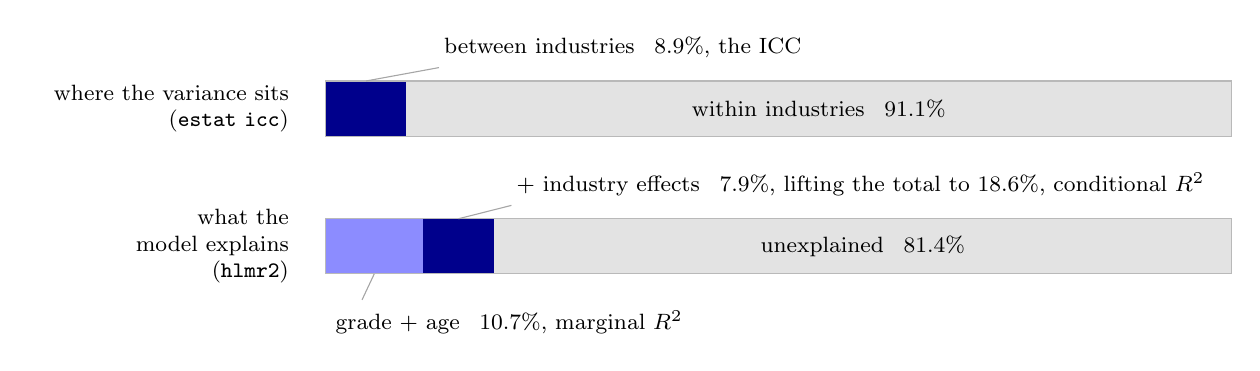
\begin{tikzpicture}[x=1.15mm, y=1cm, font=\footnotesize]
% top bar: where the variance sits (estat icc)
\node[anchor=east, align=right, text width=3.2cm] at (-3,2.1)
  {where the variance sits\\(\texttt{estat icc})};
\fill[blue!55!black] (0,1.75) rectangle (8.9,2.45);
\fill[gray!22] (8.9,1.75) rectangle (100,2.45);
\draw[gray!55, thin] (0,1.75) rectangle (100,2.45);
\node at (54.45,2.1) {within industries \enskip 91.1\%};
\node[anchor=south west] at (12,2.62) {between industries \enskip 8.9\%, the ICC};
\draw[thin, gray!70] (4.45,2.45) -- (12.5,2.62);
% bottom bar: what the model explains (hlmr2)
\node[anchor=east, align=right, text width=3.2cm] at (-3,0.35)
  {what the model explains\\(\texttt{hlmr2})};
\fill[blue!45] (0,0) rectangle (10.7,0.7);
\fill[blue!55!black] (10.7,0) rectangle (18.6,0.7);
\fill[gray!22] (18.6,0) rectangle (100,0.7);
\draw[gray!55, thin] (0,0) rectangle (100,0.7);
\node at (59.3,0.35) {unexplained \enskip 81.4\%};
\node[anchor=north west] at (0,-0.35) {grade + age \enskip 10.7\%, marginal $R^2$};
\draw[thin, gray!70] (5.35,0) -- (4,-0.33);
\node[anchor=south west] at (20,0.87) {+ industry effects \enskip 7.9\%, lifting the total to 18.6\%, conditional $R^2$};
\draw[thin, gray!70] (14.65,0.7) -- (20.5,0.87);
\end{tikzpicture}
\caption[Two reads of the same wage variance]{The same fitted model, cut two ways, with different denominators: the ICC partitions residual variance after the fixed predictors, while the $R^2$ summary includes variation in their fitted contribution. The top bar splits it by level: 8.9\% sits between industries, and that sliver is all a site-style ranking has to work with. The bottom bar splits it by explanation: grade and age account for 10.7\%, the industry effects add 7.9\%, and the rest is individual variation no ranking will touch.}
\label{fig:ch07-viz-varsplit}
\end{figure*}

Use the ICC to describe clustering, then examine uncertainty in the site estimates before deciding whether to rank them. A small ICC can coexist with precisely estimated site differences when sites are large; a large ICC can coexist with uncertain rankings when sites are small. In this adjusted wage model, the ICC describes the share of residual variation between industries after accounting for grade and age. For a program scorecard, also examine site sample sizes, intervals around site estimates, and sensitivity to the adjustment variables. Those checks address whether neighboring ranks are distinguishable, which the ICC alone cannot tell you.\marginnote{\texttt{hlmr2} covers linear mixed models fit by \texttt{mixed}. For random-slope models its summary ignores covariances and is an approximation; consult the package's output note before interpreting it.}

Shrinkage in \S\ref{sec:shrink} pulls every small site toward one common mean, whatever kind of site it is, and that is its limit. Fay-Herriot small-area estimation \parencite{fay1979estimates,rao2015small} instead uses the multilevel machinery of this section to pull each site toward the mean of sites like it\marginnote{Pulling each site toward the mean of sites like it is closer to how statistics offices produce the small-area numbers policymakers already cite.}. You pay for that in assumptions: the estimate is only as good as the covariate model behind it, so you trade assumption-light shrinkage for a stronger estimate that depends on a specification a reviewer can question.

In the applied example below we run the chapter's safeguards through a single quarterly scorecard, in the order the calendar requires.

\begin{appliedexample}[One quarterly scorecard, four safeguards]\label{ae:ch07-scorecard}
\textbf{Scenario.} A caregiver-support program runs at fifty sites, most of them small. Each quarter the evaluator ships one scorecard: an engagement score from a six-item survey scale, a completion rate per site, and a population claim about the families served. The board wants a site ranking; the director wants to know whether next year's evaluation can detect the improvement the program hopes for.

\medskip
\textbf{Applying the checks.} At the pilot, inspect the survey items and their coding before deciding whether to revise the engagement score. Before making a population claim, identify the target population and sampling design, then compare the estimate with and without the supplied weights. For site comparisons, examine caseloads and adjusted rates together with their uncertainty; discuss which differences are useful enough to act on. During planning, calculate power for effects that would change the program decision and revisit the design if those effects are hard to detect. Prediction intervals can inform planning for individual cases when new cases resemble the calibration sample, while the ICC describes clustering rather than authorizing a ranking. Record what each check showed and the decision it informed in the scorecard's methods note.
\end{appliedexample}

\paragraph{Where this leaves you.} You can now examine how a score was constructed, check the design behind a weighted estimate, and report small-site rates with appropriate uncertainty. Power calculations help you plan the study before enrollment, while prediction intervals and variance components address different questions about individual outcomes and clustering. These checks document the limits of the numbers you will compare in Chapter~\ref{ch:claims}; none removes the need to match the eventual claim to the study design.

\section*{Exercises}\addcontentsline{toc}{section}{Exercises}
\begin{enumerate}
  \item \emph{Try it on your own data.} Pick a multi-item scale you already collect, run \texttt{alpha} with the \texttt{item} option, and read the item-rest correlations: flag every item below 0.30 and confirm that dropping the worst one raises the whole-scale alpha in the \enquote{alpha if item dropped} column.
  \item Rerun \texttt{ch07\_trust.do} on the NHANES~II example, but before the weighted line predict, out loud, whether \texttt{svy: mean highbp} will land above or below the unweighted 0.4229; then run it and check your call against the 0.3687 the chapter reports.
  \item Break the shrinkage code on purpose: change the caseload for one site to a negative number, rerun the beta-binomial block, and confirm that the resulting \texttt{pshrunk} becomes nonsensical, then add an \texttt{assert n > 0} tripwire that catches the bad input before the estimator runs.
  \item Using \texttt{power twomeans} with the chapter's control mean of 50 and \texttt{sd(10)}, find the total sample size that first pushes the 3-point effect to 0.80 power, and report whether it falls above or below the budgeted $N=300$.
  \item Simulate a single five-person site with three successes, place it among the 50 simulated sites, and compare its raw rate of 0.60 against its shrunken rate: explain in one sentence why empirical Bayes pulls it so far toward the grand mean of 0.195.
  \item Run \texttt{rateshrink} with \texttt{rel()} on the 50-site draw and confirm the reliability identity by hand: for the most-shrunken site, check that its reliability equals $n/(n+\alpha+\beta)$ from the header's $\alpha$ and $\beta$, and say in one sentence why a site pulled halfway to the grand mean has a reliability near 0.5.
  \item Write the one-sentence translation a program officer could act on for each of the chapter's four safeguards, one clause of finding and one of license, using the chapter's own numbers: the 0.79 alpha, the 0.37 weighted rate, site~26's shrunken 0.160, and the 41\% power at a 2-point effect.
\end{enumerate}
